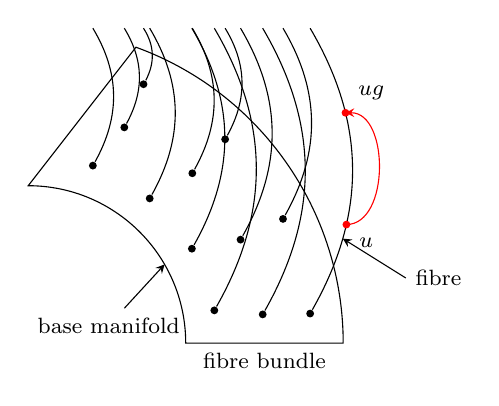
\begin{tikzpicture}[>=stealth, every node/.style={font=\footnotesize}]
    % manifold
    \draw(2,0)--(4,0)node[midway,below]{fibre bundle}arc(0:70:4)--(90:2)arc(90:0:2)--cycle;
    \draw[->] (20:1.3)node[below,xshift=-2mm]{base manifold}--(30:2);

    % fibres
    \begin{scope}[bend right]
        \foreach \i[count=\x] in {10,30,50,70}
        {\node(a\x)[circle,fill,inner sep=1pt]at (\i:2.4){};
        \draw(a\x)to(a\x|-0,4);}

        \foreach \i[count=\x] in {7,26,46,66}
        {\node(b\x)[circle,fill,inner sep=1pt]at (\i:3){};
        \draw(b\x)to(b\x|-0,4);}

        \foreach \i[count=\x] in {6,26,46,66}
        {\node(c\x)[circle,fill,inner sep=1pt]at (\i:3.6){};
        \draw(c\x)to(c\x|-0,4);}


        \path(c1)to coordinate[near start](d)(c1|-0,4);

        \path(c1) to coordinate[ pos=0.3 ](x)(c1 |- -0,4);
        \path(c1) to coordinate[ pos=0.7 ](y)(c1 |- -0,4);
    \end{scope}

    \draw[<-](d)--+(0.8,-0.5)node[right]{fibre};

    % u and ug
    \draw (x) node [red, circle, fill, inner sep=1pt, label=below right:{ $u$ }] {};
    \draw (y) node [red, circle, fill, inner sep=1pt, label=above right:{ $u g$ }] {};
    \draw[->, red] (x) to [ bend right=90 ] (y);
\end{tikzpicture}
